%19/02 - José Manuel Rodríguez
\part{Proteómica y Metabolómica}
\chapter{Introducción a la proteómica y la espectrometría de masas}
\section{Introducción}
El \textbf{proteoma} se define como el conjunto completo de proteínas que se expresan, o pueden expresarse, a partir del genoma de una célula, tejido u organismo en un momento y condición específicos. La \textbf{proteómica}, por su parte, es la disciplina científica que estudia el proteoma mediante técnicas sistemáticas para identificar, cuantificar y caracterizar proteínas. Entre las herramientas más utilizadas en proteómica se encuentran la electroforesis, la espectrometría de masas (MS), la resonancia magnética nuclear (RMN), la microscopía óptica y electrónica, y la espectroscopía infrarroja por transformada de Fourier, entre otras.

\subsection{Análisis de proteínas por electroforesis}
La electroforesis es una técnica clásica de separación de proteínas basada en su carga eléctrica y masa molecular. En este método, las proteínas se separan en un gel según su punto isoeléctrico (pI), que es el pH al cual una proteína tiene una carga neta cero. Posteriormente, se realiza una segunda separación en función del peso molecular. Esta técnica ha sido fundamental en la proteómica "clásica" y sigue utilizándose para la validación de biomarcadores.

Tras la separación, el gel puede cortarse para aislar las proteínas de interés, las cuales se someten a una digestión con proteasas (como la tripsina) para generar péptidos. Estos péptidos pueden analizarse posteriormente mediante espectrometría de masas.

Sin embargo, la electroforesis presenta limitaciones: no es automática, tiene baja reproducibilidad y no es adecuada para proteínas grandes o hidrofóbicas. Además, suele ser efectiva solo para proteínas altamente abundantes. Estas limitaciones llevaron al desarrollo de la proteómica "Bottom-Up", que supera muchos de estos problemas.

\section{Proteómica "Bottom-Up"}
La proteómica "Bottom-Up" es un enfoque moderno que se basa en la digestión de proteínas en péptidos, seguida de su análisis mediante cromatografía líquida acoplada a espectrometría de masas (LC-MS). Este método es más sensible, reproducible y adecuado para el análisis de proteínas de baja abundancia.

\subsection{Digestión tríptica}
El primer paso en la proteómica "Bottom-Up" es la digestión de las proteínas. Las proteínas, en su estado nativo, están plegadas y pueden contener enlaces disulfuro que estabilizan su estructura. Para facilitar su análisis, las proteínas se desnaturalizan utilizando agentes como el dodecilsulfato sódico (SDS), que rompe los enlaces disulfuro y despliega las proteínas. Una vez desnaturalizadas, se someten a una digestión con tripsina, una enzima que corta específicamente después de los residuos de lisina (K) y arginina (R), generando péptidos de tamaño adecuado para su análisis por espectrometría de masas.

\subsection{Fraccionamiento para reducción de complejidad}
Tras la digestión, los péptidos resultantes pueden fraccionarse para reducir la complejidad de la muestra. Esto es especialmente útil en muestras que contienen múltiples proteínas o especies. El fraccionamiento puede realizarse mediante técnicas como la cromatografía de fase reversa, donde los péptidos se separan según su hidrofobicidad. Este paso permite una introducción más controlada y ordenada de los péptidos en el espectrómetro de masas.

\subsection{Cromatografía líquida y espectrometría de masas}
Los péptidos, fraccionados o no, se introducen en un sistema de cromatografía líquida (LC). Aquí, los péptidos se separan en función de su interacción con la fase estacionaria, lo que permite su elución en tiempos específicos. A medida que los péptidos salen de la columna cromatográfica, se ionizan mediante técnicas como la ionización por electrospray (ESI), formando gotitas cargadas que contienen los péptidos ionizados. A medida que el solvente se evapora, los péptidos ionizados entran en el espectrómetro de masas.

\subsubsection{Componentes del espectrómetro de masas}
Un espectrómetro de masas consta de los siguientes componentes principales:
\begin{itemize}
\item \textbf{Sistema de introducción de muestras}: Introduce los péptidos ionizados en el espectrómetro.
\item \textbf{Cámara de ionización}: Aquí, los péptidos se ionizan. Una de las técnicas más comunes es la ionización por electrospray (ESI).
\item \textbf{Analizador}: Determina la relación masa-carga (m/z) de los iones. Existen diferentes tipos de analizadores, como los de cuadrupolo, tiempo de vuelo (TOF) y trampa de iones.
\item \textbf{Detector}: Registra la masa y la intensidad de los iones detectados.
\end{itemize}

\begin{figure}[h]
\centering
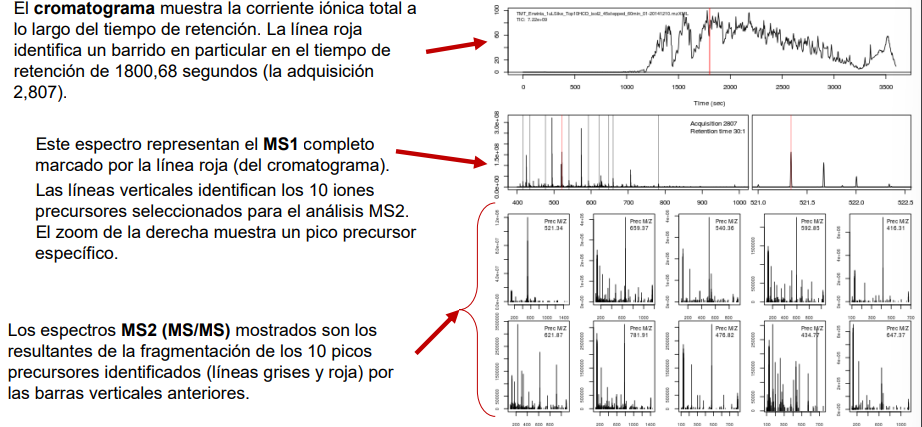
\includegraphics[width = \textwidth]{figs/espectro-analisis.png}
\caption{La figura superior indica el cromatograma obtenido. Primero hay un tiempo de retención con la intensidad encontrada de toda la carga iónica recibidas. A partir de un tiempo de retención señalado con la línea roja, empieza el tiempo de adquisición. El MS1 (panel central) es la ampliación de la línea roja del cromatograma. Cada línea vertical indica la masa detectada con sus intensidades. La parte derecha es un zoom de la línea roja. El MS1 se genera por cada péptido encontrado. Para este ejemplo, se cogen los iones marcados en gris y rojo y se fragmentan. Se saca la masa, carga e intensidad por cada uno de los iones en el segundo analizador. }
\end{figure}

La siguiente imagen muestra una representación de un LC-MS. A partir de un determinado tiempo de retención, hay una serie de masas cargas de los péptidos con una intensidad asociada a cada uno. Para diferentes tiempos de retención hay diferentes picos del espectrómetro.

\begin{figure}[h]
\centering
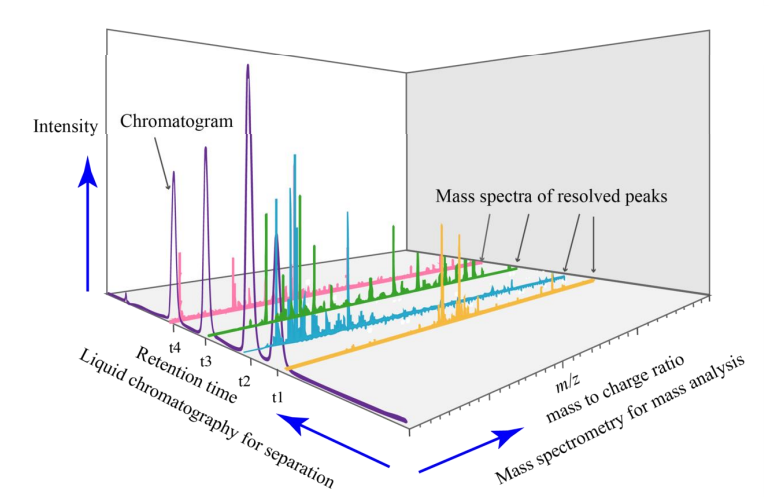
\includegraphics[width = \textwidth]{figs/lc-ms.png}
\end{figure}

Se tienden a coger los picos con mayor intensidad, ya que el resto son ruido del espectrómetro. Se sabe que a la hora de tener los péptidos, hay unos iones que van del extremo N-terminal al C-terminal y otros que van en sentido contrario. Estos iones van calculando la masa acumulativa. De esta forma se pueden saber los aminoácidos que componen el espectro.

\begin{figure}[h]
\centering
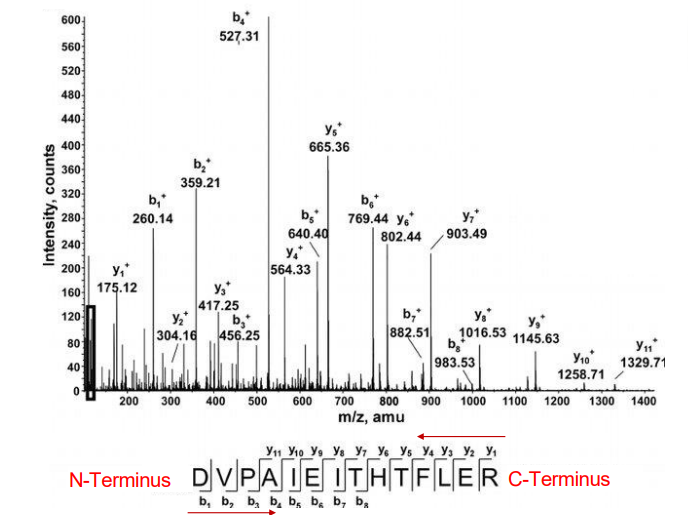
\includegraphics[width = 0.6\textwidth]{figs/fragmentacion-msms.png}
\end{figure}

\subsection{Adquisición de datos}
La adquisición de datos en espectrometría de masas puede realizarse de dos formas principales:
\begin{itemize}
\item \textbf{Adquisición dependiente de datos (DDA)}: En este modo, los iones más abundantes detectados en el espectro MS1 se seleccionan para su fragmentación, generando espectros MS2. Este proceso se repite secuencialmente para múltiples iones.
\item \textbf{Adquisición independiente de datos (DIA)}: En este modo, se fragmentan regiones específicas del espectro MS1, independientemente de la intensidad de los iones. Esto permite la detección de iones de baja abundancia, aunque puede resultar en espectros MS2 más complejos debido a la co-fragmentación de múltiples péptidos.
\end{itemize}

\begin{figure}[h]
\centering
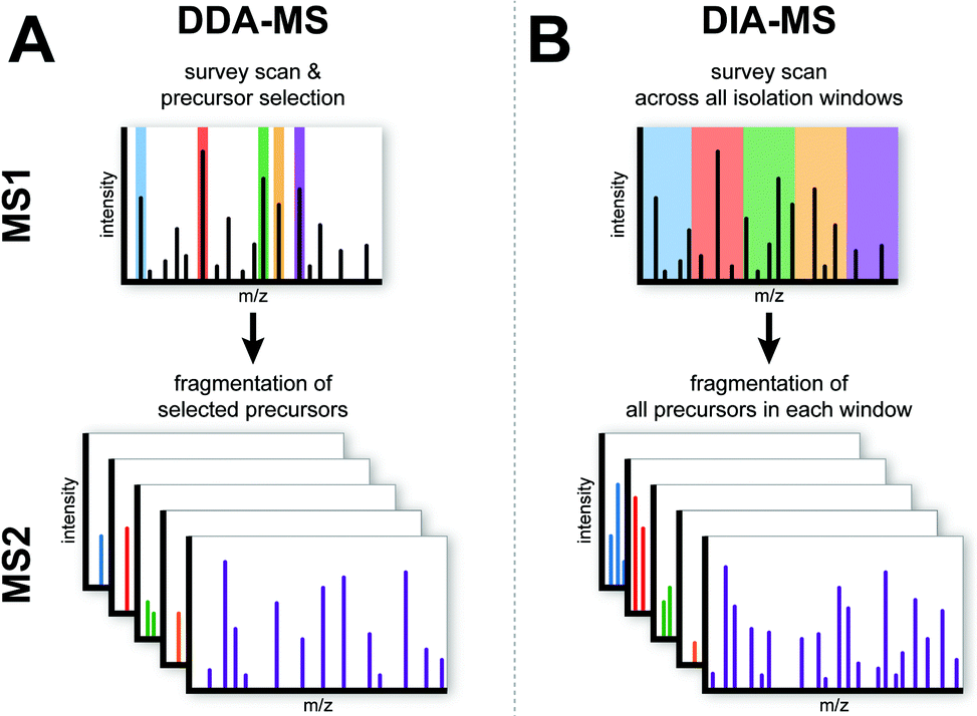
\includegraphics[width = 0.6\textwidth]{figs/data-adquisition.png}
\end{figure}

\subsection{Identificación de péptidos y proteínas}
La identificación de péptidos y proteínas se realiza comparando los espectros experimentales con bases de datos teóricas. Estas bases de datos contienen información sobre las masas y secuencias de péptidos generados in silico a partir de proteínas conocidas. Al comparar los espectros experimentales con los teóricos, se puede determinar la secuencia de aminoácidos de los péptidos y, por tanto, identificar las proteínas presentes en la muestra. Cada identificación se asocia con un score de confianza que indica la fiabilidad del resultado.

\subsection{Aplicaciones de la proteómica "Bottom-Up"}
La proteómica "Bottom-Up" tiene dos enfoques principales:
\begin{itemize}
\item \textbf{Proteómica de descubrimiento (Discovery Proteomics)}: Se utiliza para analizar proteomas completos, identificando y cuantificando proteínas de abundancia moderada a alta. Un posible ejemplo es la búsqueda de posibles biomarcadores.
\item \textbf{Proteómica dirigida (Targeted Proteomics)}: Se centra en la cuantificación de proteínas específicas, incluso en bajas abundancias. Una técnica común en este enfoque es el monitoreo de reacciones seleccionadas/múltiples (SRM/MRM), que utiliza tres analizadores de cuadrupolo para seleccionar y cuantificar péptidos específicos. Un ejemplo de aplicación es la validación de biomarcadores.
\end{itemize}

\subsubsection{Cuantificación y estándares internos}
En la cuantificación de proteínas, es crucial utilizar estándares internos para corregir variaciones en la ionización y la eficiencia de la cromatografía. Estos estándares son péptidos sintéticos con propiedades similares a los péptidos de interés, pero marcados con isótopos estables. Al comparar las áreas bajo la curva de los péptidos de interés con las de los estándares internos, se obtiene una cuantificación precisa y reproducible.

\begin{figure}[h]
\centering
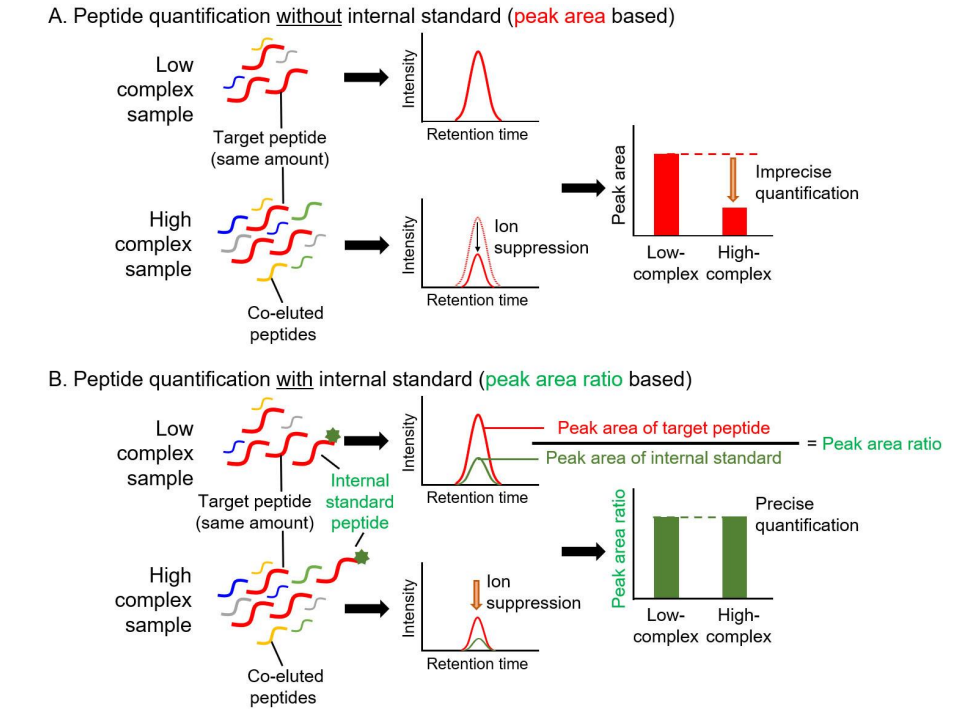
\includegraphics[width = 0.8\textwidth]{figs/internal-standard.png}
\end{figure}

%Cuando la muestra es compleja, los péptidos pueden competir causando colución. La intensidad va a disminuir al haber menos iones que se cuantificarán. La cuantificación de una muestra compleja será por tanto menor que el mismo péptido en una muestra poco compleja. Por esto, se establecen estándares internos: péptides con cualidades similares marcados. Se conoce la cantidad a priori del péptido asociado. Así, da igual si la complejidad es mucha o poca, ya que se establece la relación entre el péptido asociado y el péptido buscado. Lo que se calcula es el ratio del pico, es decir, el área del péptido buscado con el área del estándar interno. 

%21/02 - José Manuel Rodríguez
\section{Proteómica "Top-Down"}
En este caso, tenemos la proteína intacta y se calcula la masa con el espectrómetro. Se usan los mismos tipos de espectrómetros: cromatografía líquida y espectrómetro de masas. Químicamente, la muestra biológica no se desnaturaliza ni se digiere, si no que se sigue un protocolo de lisis para romper las membranas celulares. Dependiendo de las muestras y sus condiciones, las proteínas mantendrán su estructura o si están haciendo ligando, se mantendrán las relaciones. Si para esas condiciones de muestra hay alguna modificación post-traduccional, va a ser más fácil de identificar con esta técnica de Top-Down. 

Las proteínas intactas se pasan a un HPLC. Se realiza la ionización por electrospray y con el tiempo de retención y las intensidades, se obtiene la masa carga de toda la proteína (MS1). Posteriormente se fracciona en determinados puntos dentro de la proteína. Es más fácil obtener la estructura de la proteína. El MS2 permite ver la estructura de fragmentos de la proteína. 

En el caso del Bottom-Up, tenemos toda la proteína y se hace una digestión tríptica. Los péptidos se ionizan, y esos fragmentos ionizados son los que detectará el MS. En Top-Down, la proteína intacta se ioniza. Al fragmentar para el MS2, hay trozos y fragmentos de los iones con una conformación de la proteína más larga, siendo así más fácil ver la estructura completa. 

Comparando las dos técnicas en proteómica:
\begin{table}[h]
\centering
\begin{tabular}{p{4cm}|p{5cm}p{5cm}}
Aspecto & Top-Down & Bottom-Up \\ \hline
Tamaño de las proteínas & Adecuado para proteínas pequeñas y medianas & Adecuado para todo tamaño, especialmente proteínas grandes \\
Equipos & Instrumentos de alta resolución & Instrumentos más accesibles \\
Sensibilidad & Menor, difícil para proteínas en baja abundancia & Mayor sensibilidad \\
Complejidad computacional & Alta, espectros más difíciles de interpretar & Menor, espectros de péptidos más sencillos \\
Cobertura & Cobertura completa de la proteína & Cobertura parcial (depende de la digestión) \\
Manejo de mezclas complejas & Difícil para mezclas de muchas proteínas & Más fácil, adecuado para muestras complejas \\
Detección de PTMs & Precisa, localización directa en la proteína intacta & Puede perder algunas PTMs, pero identifica modificaciones en péptidos \\
Preparación de muestras & Más compleja, requiere proteínas intactas & Más sencilla, con digestión enzimática
\end{tabular}
\end{table}

\begin{figure}[h]
\centering
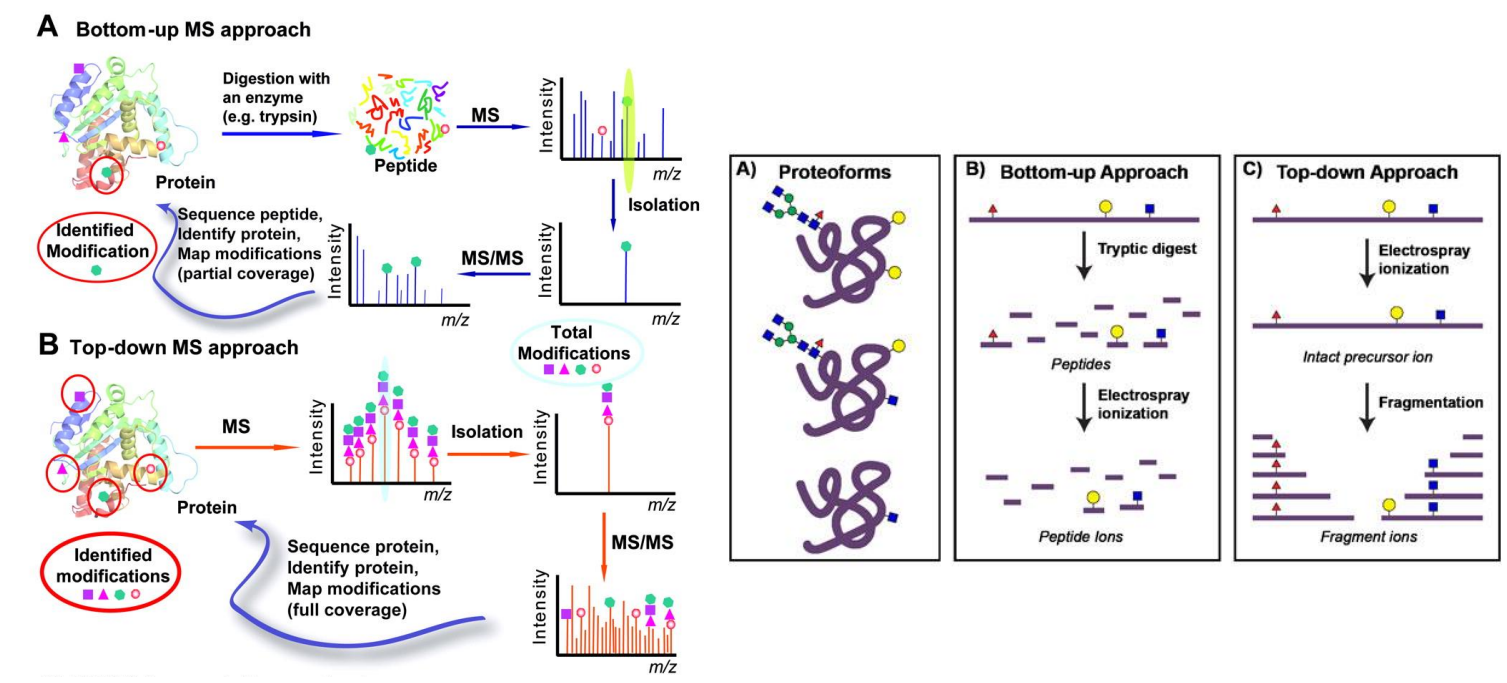
\includegraphics[width = 0.9\textwidth]{figs/topdown-vs-bottomup.png}
\end{figure}

\chapter{Identificación de péptidos mediante espectrometría de masas}
Las máquinas actuales generan millones de espectros MS/MS en muy poco tiempo. No se pueden interpretar manualmente, siendo necesario usar herramientas computacionales. 
Las estrategias más utilizadas para identificar péptidos mediante MS/MS son:
\begin{itemize}
\item \textbf{Secuenciación \textit{de novo}}: Consiste en obtener la secuencia del péptido directamente a partir del espectro.
Se usa en casos donde el genoma del organismo no está (o sólo parcialmente) secuenciado. La
secuencia se infiere directamente del espectro sin ayuda de una base de datos de referencia.
También se usa para identificar o caracterizar modificaciones postraduccionales.

\item \textbf{Búsqueda contra bases de datos}: Se identifica el péptido en la base de datos a partir del espectro MS/MS. Para ello se hace una "correlación" entre el espectro MS/MS obtenido experimentalmente y los espectros teóricos generados a partir de las secuencias de los péptidos en la base de datos.

Los motores de búsqueda se encargan de asignar a cada espectro obtenido experimentalmente un péptido, que es el mejor candidato de una lista de los posibles péptidos en la base de datos, de acuerdo a cierta \textbf{puntuación}, que mide el \textbf{grado de similitud entre el espectro empírico y el teórico}.
A cada una de estas \textbf{parejas péptido-espectro} se les denomina \textbf{PSM} (Peptide-Spectrum Match, Asignación Péptido-Espectro). 

Denominaremos \textbf{puntuaciones simples} a aquellos algoritmos que generan una puntuación para cada PSM que es independiente de la puntuación asignada al resto de PSMs en el mismo experimento.
Los algoritmos que asignan una puntuación a cada PSM considerando el comportamiento del resto de las PSM generan puntuaciones que denominaremos \textbf{complejas}.
\end{itemize}

\section{Algoritmos de identificación de péptidos - Puntuaciones simples}
Hay varios algoritmos para poder obtener esta puntuación:
\begin{itemize}
\item \textbf{Algoritmos empíricos de puntuación}
\begin{itemize}
\item SEQUEST
\item Reginamiento de las puntuaciones SEQUEST
\end{itemize}
\item \textbf{Algoritmos basados en la probabilidad del emparejado}
\begin{itemize}
\item Mascot
\item Andromeda
\end{itemize}
\item \textbf{Algoritmos basados en la probabilidad del candidato entre el resto de los candidatos}
\begin{itemize}
\item p-value y e-value
\item X!Tandem
\item MSFragger
\end{itemize}
\end{itemize}

\subsection{Algoritmos empíricos de puntuación}
SEQUEST mide el grado de similitud entre el espectro adquirido y el espectro teórico. Todos los péptidos tienen una suma de masas que concuerdan con el espectro y un rango de posible error. Tras obtener la lista de los fragmentos que coinciden con la suma de masas, se crea un espectro teórico y se compara uno y otro. En caso de SEQUEST, es ver que los picos de fragmentos coincidan con ellos. El score da la suma de cada fragmento con un margen de error y ver si coincide. Con esto se selecciona el fragmento con mayor similitud y nos quedamos con él. 

A partir de esto, aparecen otras puntuaciones de refinamiento. Un ejemplo es $\Delta C_n$. Este algoritmo indica el valor de la diferencia entre las puntuaciones ordenadas. SI el segundo candidato en puntuación es muy bajo (hay una gran diferencia), nos podemos fiar más del primer candidato por el score obtenido. Puede suceder que el valor de $\Delta C_n$ sea alto, pero la puntuación base sea baja. O al revés, que haya muy poca diferencia entre puntuaciones, pero éstas sean muy altas. 

Otro refinamiento de SEQUEST es $cXcorr$. Éste refinamiento depende de la masa: a mayor masa, más aminoácidos, habiendo más fragmentos que emparejar y un valor más elevado de Xcorr. También depende de la carga, ya que a igual m/z, los péptidos con más carga tienen más aminoácidos, por lo que el valor de Xcorr también tiende a ser más alto. Por tanto, Xcorr da prioridad a los péptidos de mayor masa y de mayor carga. Una forma de corregir este efecto es con cXcorr, que se hace independiente de la longitud del péptido.

\subsection{Probabilidad en el emparejado}
\paragraph{Mascot}
Mascot puntúa el emparejamiento entre una secuencia y un espectro MS/MS calculando la probabilidad de que el emparejamiento sea un evento aleatorio. El algoritmo no se ha publicado. Utiliza la puntuación Ion Score (IS) que se define como $IS = -10 \cdot \log P$, donde $P$ es la probabilidad de que la coincidencia observada entre el espetro teórico y el experimental sea un evento aleatorio. El IS refleja la calidad del emparejamiento. Cuanto más bajo sea P, mayor será el puntaje; es decir, una puntuación alta es indicativo de un emparejamiento más fiable entre el espectro experimental y la secuencia teórica. Se trata de un software comercial de uso gratuito para búsquedas pequeñas.

\paragraph{Andromeda}
Andromeda es un motor de búsqueda de péptidos que utiliza un concepto semejante a Mascot. El algoritmo ha sido publicado. Se basa en el cálculo de la probabilidad binomial de tener un número de fragmentos en el espectro que coincidan al azar. Andromeda se ofrece como “software” libre que puede funcionar de forma independiente o integrada dentro del paquete MaxQuant.

%26/02 - José Manuel
\subsection{Probabilidad del candidato}
\subsubsection{p-value y función de densidad de probabilidad (FDP)}
Para calcular el p-valor (p-value) se tienen en cuenta las puntuaciones obtenidas por todos los candidatos de la base de datos contra los que se compara un determinado espectro MS/MS.
El p-value de una puntuación x se define como la probabilidad de que el espectro encuentre una PSM de puntuación igual o mejor que x. Esta probabilidad se puede obtener a partir de la Función de Densidad de Probabilidad (FDP o Probability Density Distribution). Para generar la FDP se ordenan las puntuaciones de menor a mayor (1), se construye un histograma y se ajusta a una función empírica (2), se normaliza la función para que el área sea la unidad (3) y se calcula el área por encima de la puntuación (s) dada. 

\begin{figure}[h]
\centering
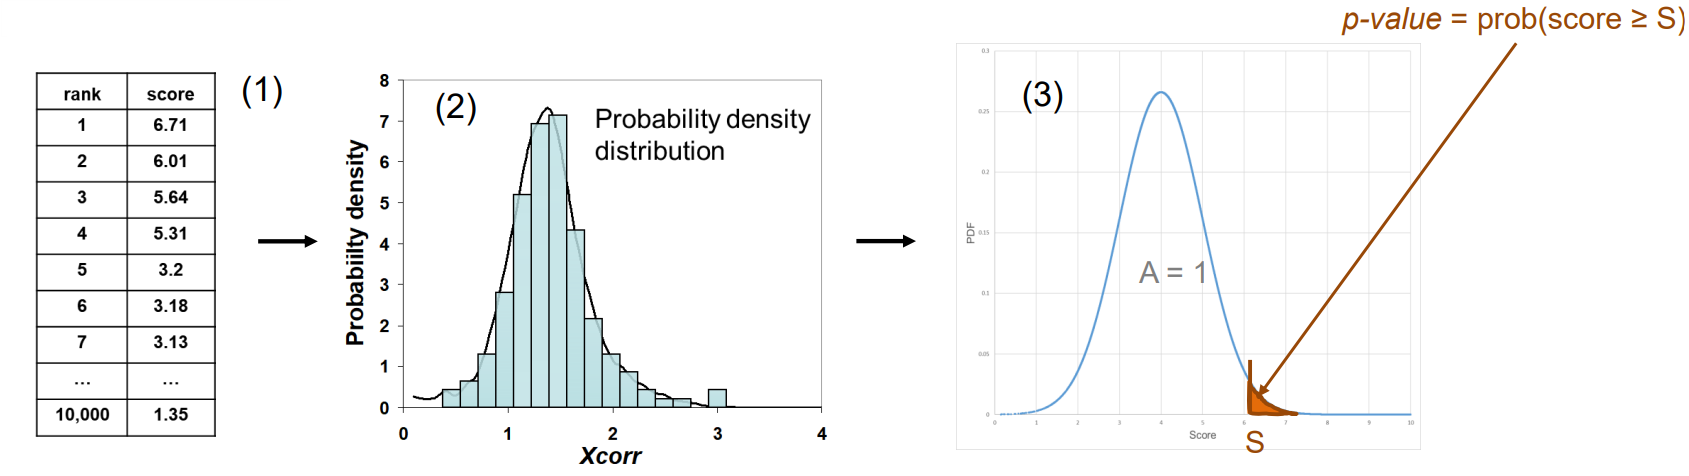
\includegraphics[width = 0.9\textwidth]{figs/fdp.png}
\end{figure}

\subsubsection{Valor esperado (e-value)}
Supongamos que obtenemos una PSM con p-value = 0.001 después de buscar contra N = 1000 secuencias candidatas. ¿Se puede considerar este resultado significativo?
La probabilidad de obtener una o más coincidencias con una probabilidad p o menor cuando el evento se repite N veces es igual a la probabilidad de no tener N coincidencias con (1 - p), es decir:
$$p(\text{one or more matches with p or lower}) = 1 - (1 - p)^N \sim Np$$

Como se indica en la fórmula, cuando p es un valor pequeño, esta probabilidad se aproxima al producto de N y p. En el caso comentado, Np = 1000x0.001 = 1 y, por lo tanto, la coincidencia no es significativa. En otras palabras, esperaríamos que al menos una secuencia puntuaría con p = 0.001 por puro azar.

El valor esperado (e-value o expectation value) se define como el producto de N por p, y mide el número esperado de coincidencias con un valor p que se obtendría cuando el espectro MS/MS se busca contra N candidatos.

$$e = N \cdot p$$

El e-value es una forma compacta de calcular la probabilidad real de forma aproximada, y da una idea más realista de la significatividad de una PSM.

\subsubsection{X!Tandem}
X!Tandem es un motor de búsqueda que usa una puntuación llamada hyperscore (HS).
$$HS = (\sum^n_{i = 0} I_i P_i) N_b!N_y!$$
La puntuación HS tiene en cuenta la intensidad de los fragmentos que coinciden entre el espectro observado y el teórico, y el número de iones “b” e iones “y” asignados. Además, X!Tandem calcula el p-value asociado al HS para determinar si una identificación es correcta o no.

\subsubsection{MSFragger}
MSFragger es un motor de búsqueda ultrarrápido que cuya puntuación y modelado probabilístico son muy parecidos a X!Tandem. La búsqueda ultrarrápida se consigue construyendo un theoretical fragment index a partir de todas las secuencias de las bases de datos. Cada fragmento en el espectro observado se compara con todos los fragmentos de la misma masa de todos los candidatos en un solo paso.

MSFragger es adecuado para cualquier análisis de proteómica de shotgun, para búsquedas sin restricciones de enzimas, búsquedas de bases de datos “abiertas”, y para la identificación de péptidos modificados glicopéptidos. MSFragger es suficientemente rápido para ser usado incluso en un ordenador portátil.

\subsubsection{Mejor método}
Se han publicado muchas comparativas entre los diferentes motores de búsqueda, pero la situación no está clara. Algunos algoritmos funcionan mejor para ciertos péptidos, mientras que otros funcionan mejor para diferentes conjuntos de péptidos. La principal preocupación no es cuál debería usarse, sino cómo interpretar correctamente los resultados. Por lo tanto, si nos encontramos cómodos con un método de identificación de péptidos MS/MS (conocido), lo mejor es seguir usándolo. Lo importante es asegurarse de que la \textbf{validación de las identificaciones} está hecha correctamente. 

\section{Algoritmos de identificación de péptidos - Puntuaciones complejas y validación estadística}
\subsection{Validación mediante Posterior Error Probability (PEP)}
\subsubsection{PeptideProphet - Función Discriminatoria}
PeptideProphet fue en su momento un nuevo concepto de algoritmo que tiene en cuenta todos los factores que pueden influir en un buscador a la hora de decidir si una identificación es correcta. Utiliza una \textbf{función discriminatoria F} que se construye como combinación lineal de todos los factores (Xcorr, $\Delta$Cn, Ln SpRank, etc.):
$$F(x_1, x_2, \ldots, x_s) = c_0 + c_1x_1 + c_2x_2 + c_3x_3 + \ldots + c_sx_s$$
Se aplicó originalmente a las puntuaciones de Sequest, pero el concepto es de aplicabilidad universal y se ha usado con otros motores de búsqueda (Mascot, Andromeda, X!Tandem, etc). 

La función F primero se aplica a un conjunto de datos de entrenamiento (una población de espectros MS/MS bien caracterizados), con los que se optimizan los coeficientes lineales que mejor discriminan entre identificaciones correctas e incorrectas mediante un algoritmo iterativo. De esta manera se obtienen distribuciones de F separadas para las identificaciones de péptidos correctas (positivas) e incorrectas (negativas).

\begin{figure}[h]
\centering
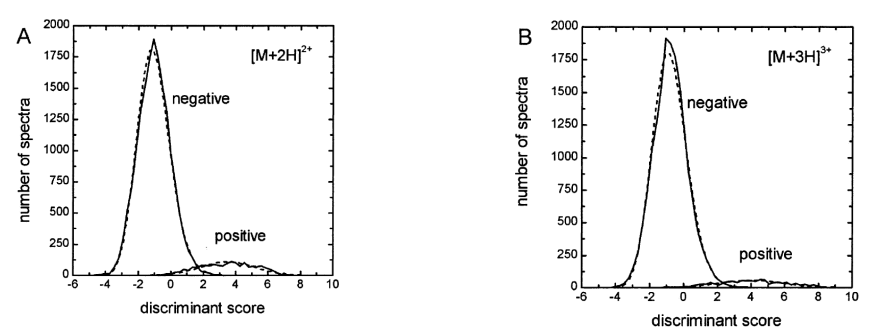
\includegraphics[width = 0.9\textwidth]{figs/peptideprophet.png}
\end{figure}

\subsubsection{Cálculo bayesiano de PEP}
Las funciones F se normalizan para convertirlas en funciones de densidad de probabilidad (PDF), de manera que la distribución de todos los péptidos se expresa como una superimposición de la de los ciertos y la de los falsos. A cada puntuación “s” se le asigna un valor PEP(s), que se define como la probabilidad de obtener un péptido falso (negativo ó N) cuando se obtiene esa puntuación “s” ("N dado s"), es decir la probabilidad bayesiana P(N/s). P(N/s) se calcula como el cociente entre la PDF de la distribución de negativos (f) y la de la distribución total (t).

\begin{figure}[h]
\centering
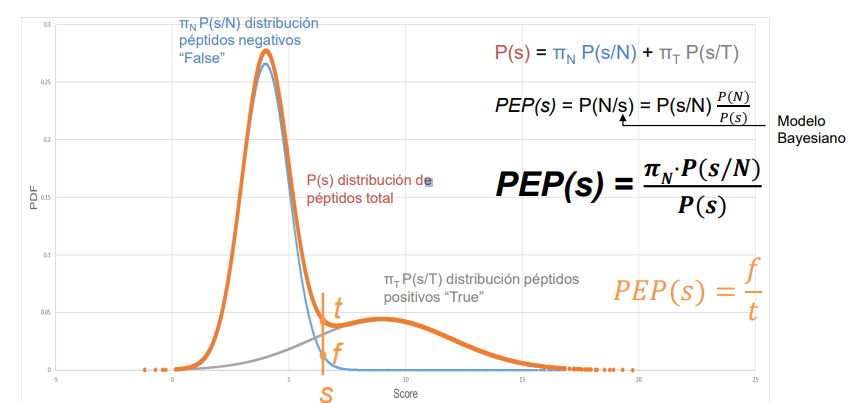
\includegraphics[width = 0.8\textwidth]{figs/bayesiano.png}
\end{figure}

\subsection{Validación mediante conceptos estadísticos globales}
\subsubsection{Tabla de contingencia}
Las tablas de contingencia se utilizan en estadística para valorar de qué manera un parámetro (en este caso la puntuación) permite discernir entre dos condiciones dadas (en este caso entre asignaciones verdaderas y falsas). En el caso ideal hay un umbral por encima del cual todas son verdaderas o todas son falsas. Idealmente, hay una separación perfecta, pero en la realidad, la separación entre ciertos y falsos es incompleta.

\begin{figure}[h]
\centering
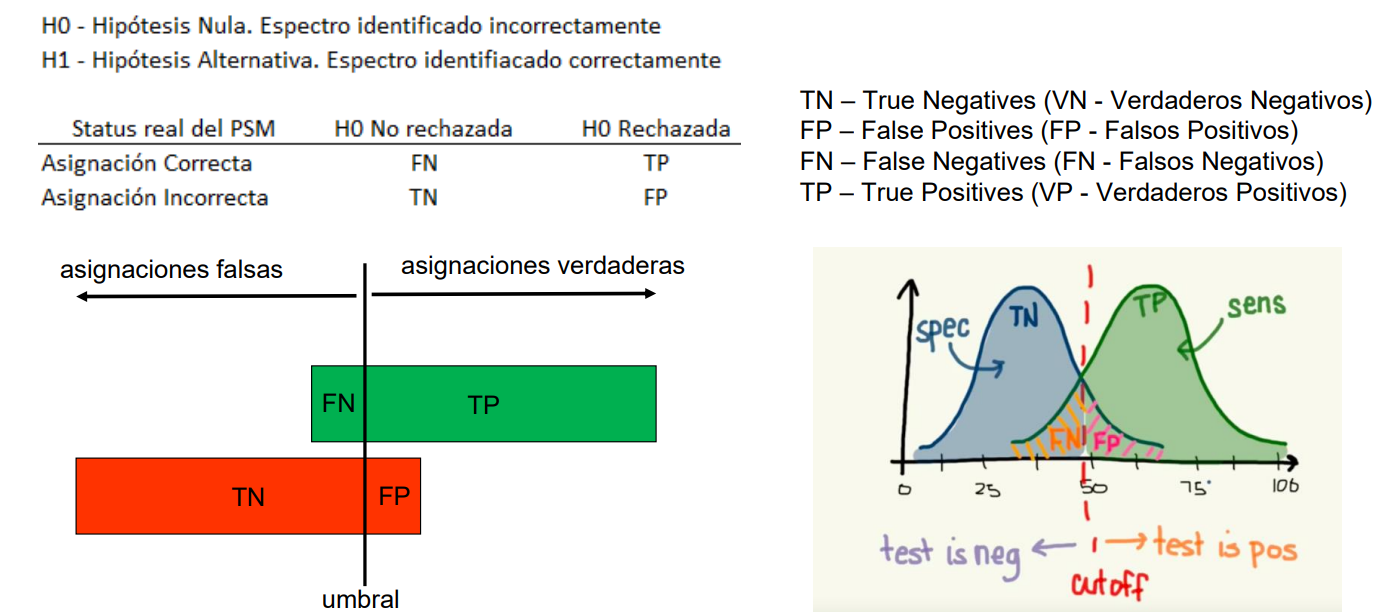
\includegraphics[width = 0.7\textwidth]{figs/contingencia.png}
\end{figure}

\subsubsection{Tasa de Falsos Positivos (FPR, False Positive Rate)}
La tasa de falsos positivos es la proporción de asignaciones consideradas correctas entre el total de asignaciones incorrectas.
$$FPR = 1 - especificidad = \frac{FP}{TN + FP}$$

La FPR equivale al p-value de la distribución global de puntuaciones.

\begin{figure}[h]
\centering
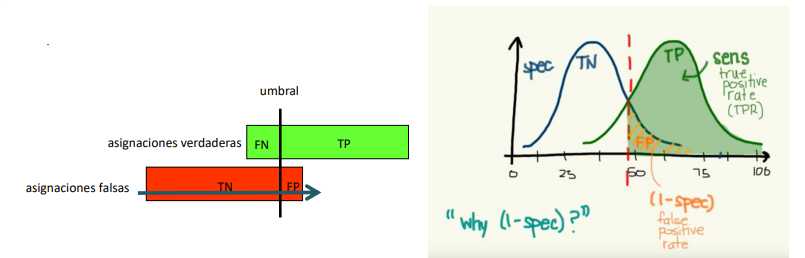
\includegraphics[width = 0.7\textwidth]{figs/fpr.png}
\end{figure}

\subsubsection{Tasa de Falsos Descubrimientos (FDR, False Discovery Rate)}
La tasa de falsos descubrimientos es la proporción de asignaciones consideradas incorrectas entre el total de asignaciones consideradas (por encima del umbral).
$$FDR = \frac{FP}{TP + FP}$$

\begin{figure}[h]
\centering
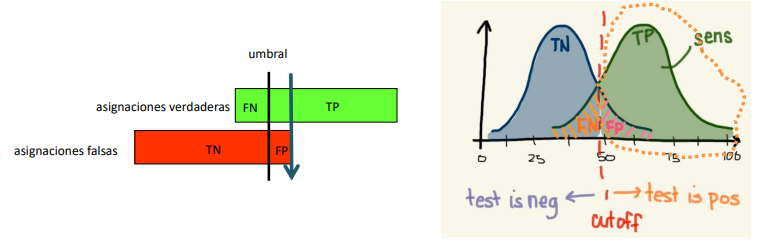
\includegraphics[width = 0.7\textwidth]{figs/fdr.png}
\end{figure}

Muy importante: la FDR es el método idóneo para corregir la FPR (ó p-value) cuando se realizan test múltiples (cuando se identifican muchos péptidos al mismo tiempo en experimentos a gran escala).

\subsubsection{Errores tipo I y errores tipo II}
\begin{itemize}
\item \textbf{Error de tipo I}, es el error que se comete cuando el investigador rechaza la hipótesis nula siendo ésta verdadera. Se evalúa calculando la probabilidad de encontrar un resultado falso positivo.
\item \textbf{Error de tipo II}, es el error que se comete cuando no se rechaza la hipótesis nula siendo falsa. Se evalúa calculando la probabilidad de encontrar un resultado falso negativo.
\end{itemize}

\begin{figure}[h]
\centering
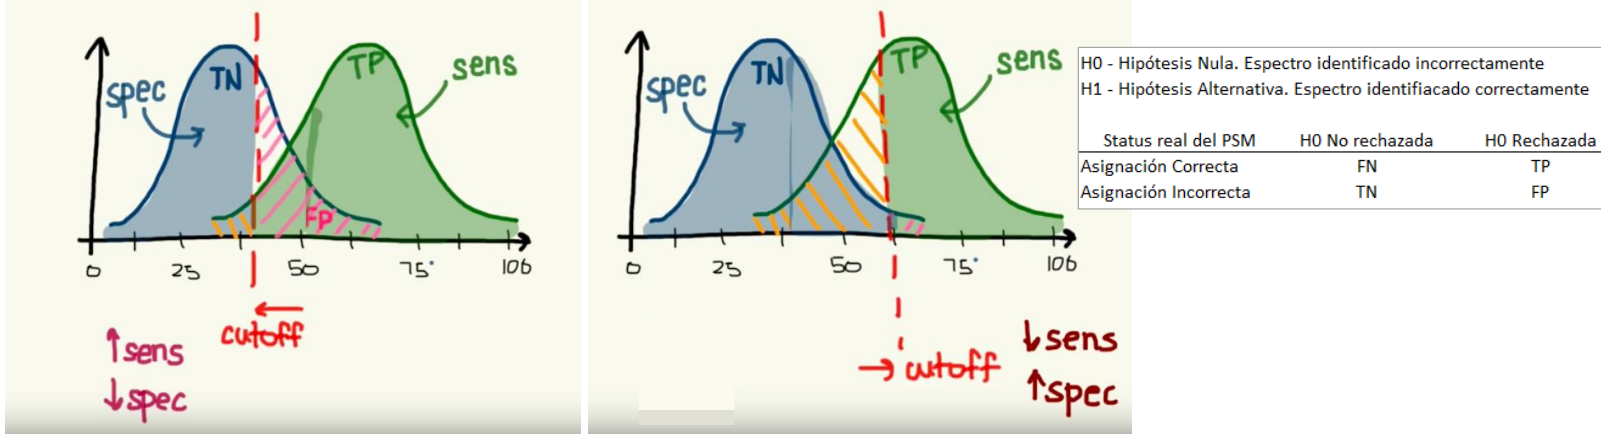
\includegraphics[width = 0.8\textwidth]{figs/error-types.png}
\end{figure}

\subsection{Estrategia Target-Decoy para el cálculo de la FDR}
\subsubsection{Uso de bases de datos señuelo o decoy}
Este es un método muy robusto y ampliamente aceptado. Se busca sobre las bases de datos de objetivo y señuelo. Se utilizan los resultados de la base de datos señuelo para estimar el número de falsos positivos en un umbral de puntaje dado.

La base de datos señuelo ("decoy") es una base de datos idéntica a la objetivo ("target") pero invirtiendo el orden de las secuencias de aminoácidos de cada proteína (C-terminal se convierte en N-terminal y viceversa), o invirtiendo las secuencias de aminoácidos de cada péptido, manteniendo los extremos básicos N-terminales (pseudoreversión).

\begin{figure}[h]
\centering
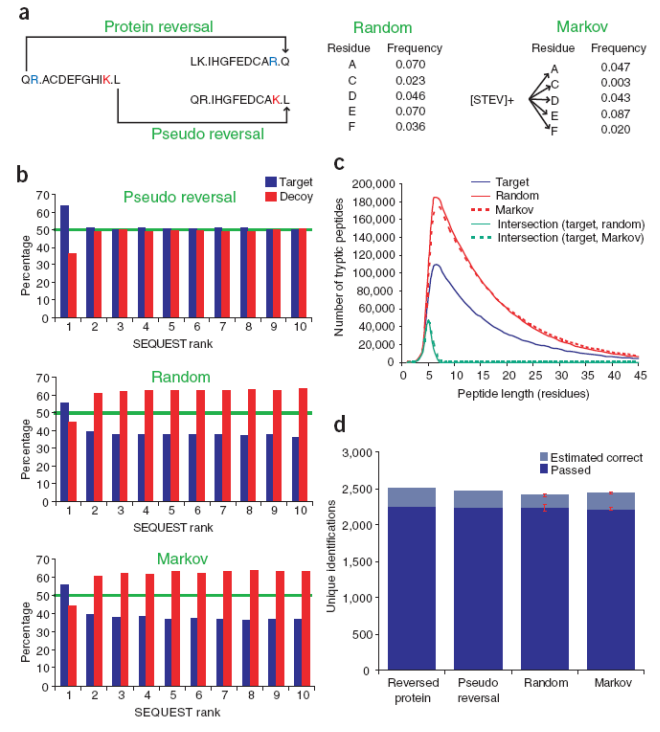
\includegraphics[width = 0.6\textwidth]{figs/decoydb.png}
\end{figure}

Las bases de datos aleatorias no se comportan de manera idéntica y sobreestiman las tasas de error (la repetición de dominios y/o motivos en la base de datos de objetivo reduce el número total de secuencias únicas).

\subsubsection{Bases de datos separadas vs bases de datos concatenadas}
En las \textbf{bases de datos separadas}, la búsqueda se realiza contra las bases de datos objetivo y señuelo de forma separada. Para cada puntuación se calcula:
\begin{itemize}
\item D: número de péptidos identificados en la base de datos señuelo (falsos)
\item T: número de péptidos identificados en la base de datos objetivo (total = ciertos + falsos)
\end{itemize}
La FDR se calcula de la siguiente manera: $FDR = D / T$.

En las \textbf{bases de datos concatenadas}, la búsqueda se realiza contra una base de datos compuesta por la base de datos señuelo, unida a la base de datos objetivo. En este caso, el número de falsos identificados en cada puntuación equivale al doble de D, y el total equivale a D + T, por lo que $FDR = 2 * D / (D + T)$

El primer método tiende a sobreestimar el número de falsos positivos, porque los espectros MS/MS de alta calidad (que corresponde a asignaciones correctas) tienes a dar puntuaciones altas en la base de datos. El segundo método evita este efecto al permitir que las secuencias objetivo y señuelo compitan por los mejores espectros, pero la FDR se calcula en una población "inflada" (contiene D). En la actualidad se prefiere el uso de bases de datos concatenadas y la FDR se calcula como $FDR = D / T$.

\subsubsection{Uso de Decoys en el modelo bayesiano: adaptación de PeptideProphet}
El enfoque de modelado probabilístico de PeptideProphet y la estrategia target-decoy se pueden combinar dentro de un solo marco semi-supervisado. Se utiliza un algoritmo de maximización de expectativas (EM) semi-supervisado para construir un clasificador bayesiano para la identificación de péptidos usando como falsos las puntuaciones “decoy” y como ciertos las puntuaciones “target”. Ello permite calcular la FDR además de la PEP.

\subsection{Percolator y Aprendizaje Automático}
Percolator utiliza un método de aprendizaje semi-supervisado automático iterativo, que se entrena para optimizar la separación entre asignaciones “target” y “decoy”.
Conceptualmente equivale a Peptide-Prophet (con la estrategia target-decoy), pero en vez de usar una función discriminatoria incluye los parámetros de la búsqueda utilizando algoritmos tipo machine-learning.
Entrena un algoritmo de aprendizaje automático, Máquinas de vectores de soporte (SVM), para discriminar entre PSM positivas y negativas.
Percolator calcula directamente la FDR usando la estrategia target-decoy.

\begin{figure}[h]
\centering
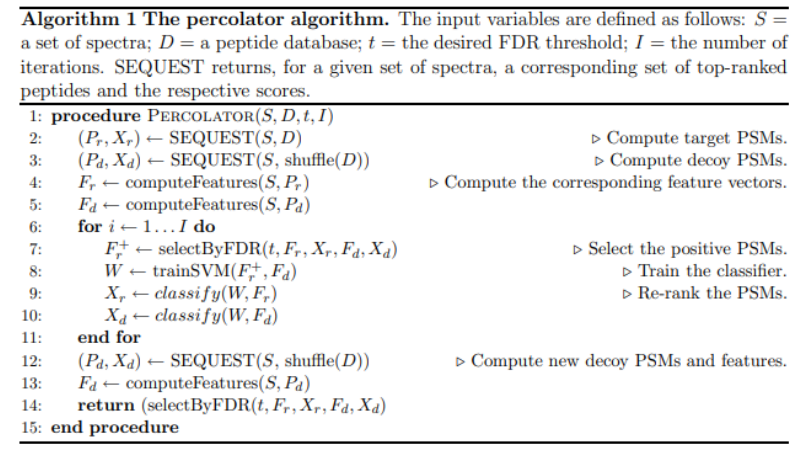
\includegraphics[width = 0.6\textwidth]{figs/percolator-pseudocode.png}
\end{figure}

\subsection{Comparativa entre PEP y FDR}
PEP y FDR son parámetros que se basan en la misma distribución de ciertos (target) y falsos (decoy). PEP mide la proporción “local” de falsos en la puntuación “s” (valor en la curva). FDR mide la proporción de falsos que tienen una puntuación igual o mayor que “s” (área de la curva). Por ello PEP se puede interpretar como la FDR “local” en la puntuación “s”. PEP es más adecuada para valorar la identificación de una PSM aislada. FDR es la que debe usarse en experimentos a gran escala cuando queremos identificar muchas PSM al mismo tiempo.
\begin{figure}[h]
\centering
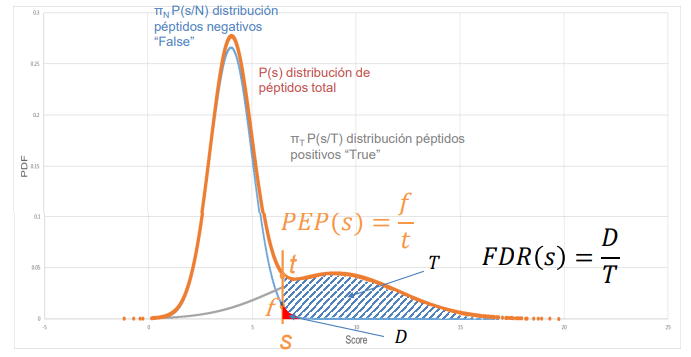
\includegraphics[width = 0.8\textwidth]{figs/pep-fdr.png}
\end{figure}